\documentclass[]{report}
\usepackage{graphicx}
\usepackage{float}
\usepackage{amsmath}
\usepackage{amsfonts}
\usepackage{wasysym}
\usepackage{listings}
\usepackage{xcolor}
\lstset{
	basicstyle=\ttfamily,
	columns=fullflexible,
	frame=single,
	breaklines=true,
	postbreak=\mbox{\textcolor{red}{$\hookrightarrow$}\space},
}
\pagenumbering{Roman}
% Title Page
\title{MCEN - 3047}
\author{Jack Goldrick}


\begin{document}
\maketitle

\section{Problem 1}

\subsection{Part A}


	\begin{figure}[H]
	\centering
	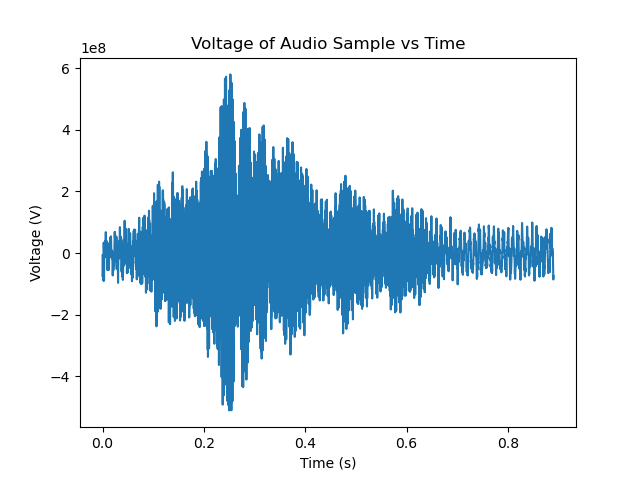
\includegraphics[width=0.7\linewidth]{../results/p1_t}
\end{figure}


\subsection{Part B}

$$ \text{LSB = 8-Bit} $$

\subsection{Part C}

$$V_fs = 709859328.0$$


\section{Problem 2}

\subsection{Part A}

\begin{figure}[H]
	\centering
	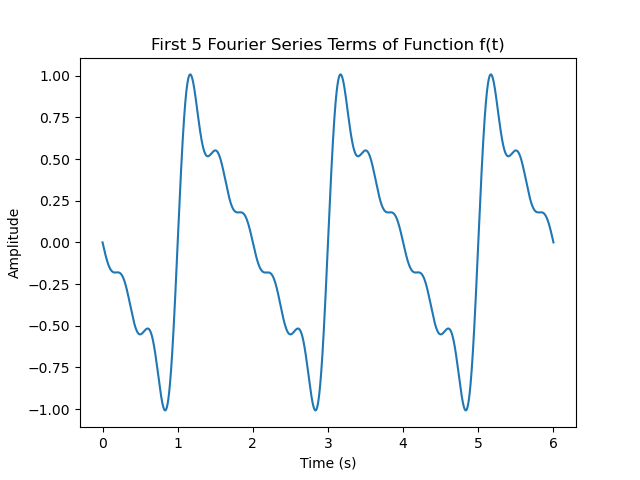
\includegraphics[width=0.7\linewidth]{../results/p2_5}
\end{figure}


\subsection{Part B}


\begin{figure}[H]
	\centering
	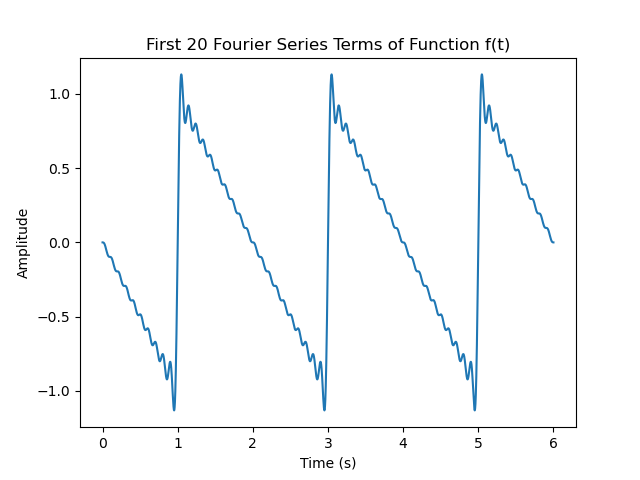
\includegraphics[width=0.7\linewidth]{../results/p2_20}
\end{figure}

\begin{figure}[H]
	\centering
	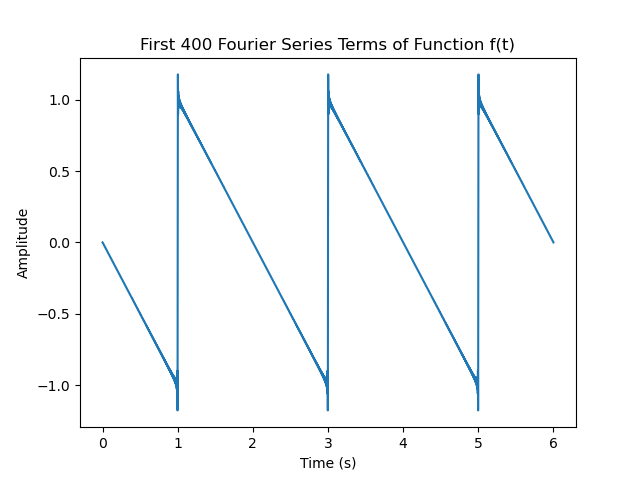
\includegraphics[width=0.7\linewidth]{../results/p2_400}
\end{figure}

\begin{figure}[H]
	\centering
	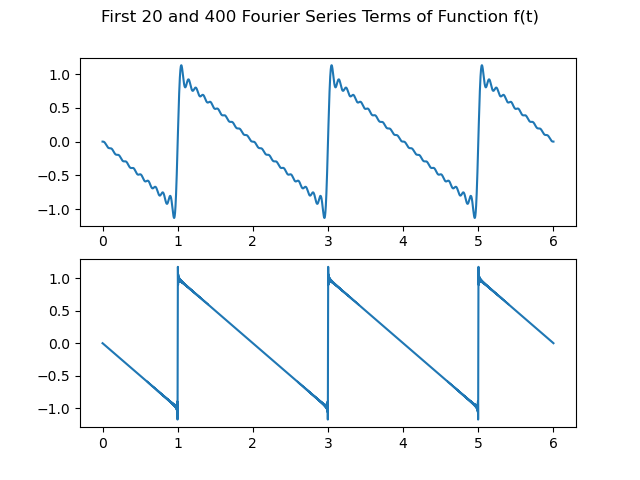
\includegraphics[width=0.7\linewidth]{../results/p2_20_400}
\end{figure}


\subsection{Part C}


\begin{itemize}
	\item The function becomes a better approximation of the cyclical ramp function  as n increases,  The function appears to become more jagged as n increases as well, better approximating digital signals, if it were one. 
\end{itemize}


\section{Problem 3}

\subsection{Part A}

\begin{figure}[H]
	\centering
	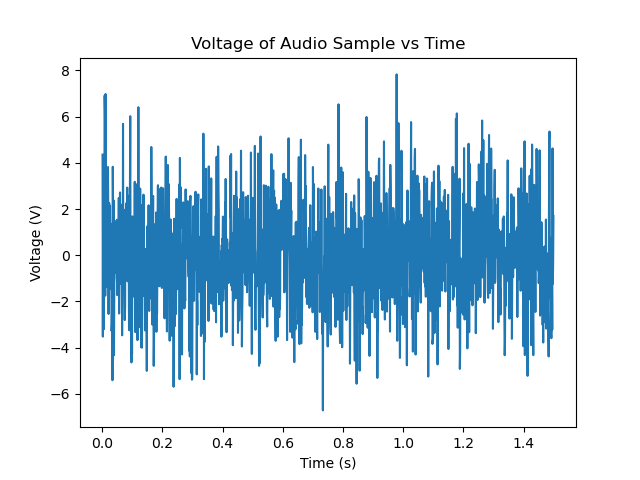
\includegraphics[width=0.7\linewidth]{../results/p3_t}
\end{figure}

\subsection{Part B}

\begin{center}
	It may be possible to get an approximation from this time-series data, however the number may be far from accurate. Thus, one cannot decipher frequency information.
\end{center}

\subsection{Part C}

\begin{figure}[H]
	\centering
	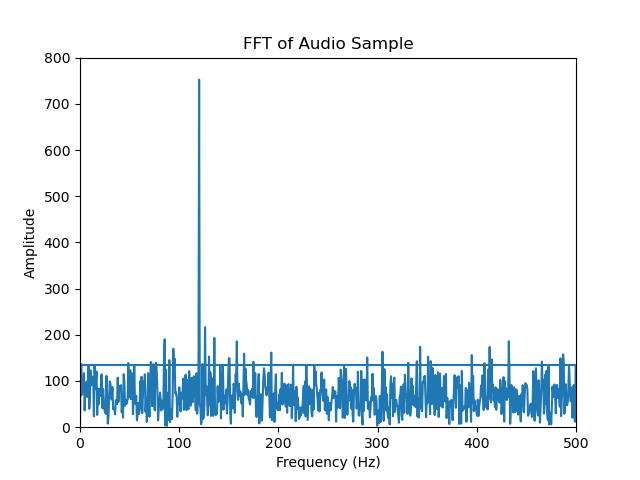
\includegraphics[width=0.7\linewidth]{../results/p3_fft}
\end{figure}


\subsection{Part D}

\begin{center}
	Frequency: 120.0800533689126
\end{center}




\newpage



\section{CODE}


\begin{lstlisting}[language=Python]


import sounddevice as sd
import scipy.io.wavfile as wav
import numpy as np
import matplotlib.pyplot as plt
import torch as tc
import pandas as pd
import os


# I Like Classes
class Set1:
	class Problem1:
		# Calculates the Voltage Range of the DAQ and the Least Significant Bit
		def get_range(self, recording):
			return self.get_step(recording) * (2 ** np.ceil(self.get_nlsb(recording)))
		
		# finds the smalles difference between two samples
		@staticmethod
		def get_step(recording):
			for i in range(recording.shape[0] - 1):
				diff = np.abs(recording[i] - recording[i+1])
		
			return np.min(diff)
		
		# Calculates the bit number of least significant bit
		def get_nlsb(self, recording):
			v_max = np.max(recording)
			# print(v_max)
			return np.log2(v_max  / self.get_step(recording))
		
		def record_audio(duration=7, fs=44100):
			recording = sd.rec(int(duration * fs), samplerate=fs, channels=2)
			sd.wait()
			return recording
		
		@staticmethod
		def get_num_samples( fs=44100, duration=7):
			return int(fs * duration)
		
		def get_time_vector(self, fs=44100, duration=7):
			num_samples = self.get_num_samples(fs=fs, duration=duration)
			# print(num_samples)
			# print("test")
			return np.linspace(start=0, stop=duration, num=num_samples)
		
		
		def plot_audio_voltage(self, recording, fs=44100):
			time =  self.get_time_vector(fs=fs, duration=len(recording)/fs)
			fig = plt.figure()
			plt.title('Voltage of Audio Sample vs Time')
			plt.xlabel('Time (s)')
			plt.ylabel('Voltage (V)')
			plt.plot(time, recording)
			plt.show()
		
		@staticmethod
		def plot_audio_fft(recording, fs=44100):
		
			# recording = recording / np.max(np.abs(recording))  # Normalize amplitude
			# db_data = 20 * np.log10(np.abs(recording) + 1e-10)
		
			fig = plt.figure()
			plt.title('FFT of Audio Sample')
			plt.xlim(0, 7000) 
			plt.ylim(0, 10e11)
			plt.xlabel('Frequency (Hz)')
			plt.ylabel('Amplitude')	
			plt.plot(np.fft.fftfreq(len(recording), 1/fs), np.abs(np.fft.fft(recording)))
			plt.show()
		
		def run(self, cat=False):
		
			if cat:
				sample_rate, recording = wav.read('../../data/freyja.wav', 'rb')
				self.plot_audio_voltage(recording=recording, fs=sample_rate)
				self.plot_audio_fft(recording, fs=sample_rate)
			else:
				recording = self.record_audio()
				self.plot_audio_voltage(recording)
				self.plot_audio_fft(recording)
			
			lsb = self.get_nlsb(recording)
			print(f"LSB: {np.ceil(lsb)}")
			V_fs = self.get_range(recording)
			print(f"V_fs: {V_fs}")
	
	class Problem2:
		@staticmethod
		def compute_function(n=5,duration=6, fs=44100):
			t = np.linspace(start=0, stop=duration, num=int(fs*duration))
			ten = [(2 * np.cos(np.pi * (i+1)) * np.sin(np.pi * (i+1) * t )) / (np.pi * (i+1)) for i in range(n)]
			ten = tc.tensor(np.array(ten))
			return ten.sum(dim=0), t
		
		
		
		def plot_n_fourier_terms(self, nt=5, duration=6, fs=44100):
			ft, t = self.compute_function(n=nt, duration=duration, fs=fs)
			fig = plt.figure()
			plt.title(f'First {nt} Fourier Series Terms of Function f(t)')
			plt.xlabel('Time (s)')
			plt.ylabel('Amplitude')
			plt.plot(t,ft)
			plt.show()
		
		
		def double_plot_n_fourier_terms(self, n1=20, n2=400, duration=6, fs=44100):
			f1, t = self.compute_function(n=n1, duration=duration, fs=fs)
			f2, t = self.compute_function(n=n2, duration=duration, fs=fs)
			fig, axs = plt.subplots(2)
			fig.suptitle('First 20 and 400 Fourier Series Terms of Function f(t)')
			axs[0].plot(t, f1)
			axs[1].plot(t, f2)
			plt.show()
		
		def run(self):
			self.plot_n_fourier_terms(nt=5)
			self.plot_n_fourier_terms(nt=20)
			self.plot_n_fourier_terms(nt=400)
			self.double_plot_n_fourier_terms()
		
		
		
	class Problem3:
		""" 1. Takes a csv file, tone, that contains audio data. 
		i. The first column is the time vector
		ii. The second column is the audio data
		2. Executes a FFT on the audio
		3. plots the timeseries data
		4. plots the FFT data
		5. Saves the plots as images
		6. calculates the frequency of the tone from the least significant bit of the DAQ 
		and voltage scale"""
		def run(self):
			df = self.read_csv()
			self.plot_audio(df)
			self.plot_audio_fft(df)
			self.calculate_peak_frequency(df)
			# self.save_plots(df)
			
		def read_csv(self, file_path='tone.csv', home=True):
			if home:
				file_path = os.path.join('../../data/', file_path)
			
				
				df = pd.read_csv(file_path)
				
				df.columns = ['time', 'audio']
			return df
		
		def plot_audio(self, df):
			fig = plt.figure()
			plt.title('Voltage of Audio Sample vs Time')
			plt.xlabel('Time (s)')
			plt.ylabel('Voltage (V)')
			plt.plot(df['time'], df['audio'])
			plt.show()
		
		def plot_audio_fft(self, df):
		
			sample_rate = (df['time'][1] - df['time'][0]) ** -1            
			fig = plt.figure()
			plt.title('FFT of Audio Sample')
			plt.xlim(0, 500) 
			plt.ylim(0, 800)
			plt.xlabel('Frequency (Hz)')
			plt.ylabel('Amplitude')
			plt.plot(np.fft.fftfreq(len(df['audio']), 1/sample_rate), np.abs(np.fft.fft(df['audio'])))
			plt.show()            
			def save_plots(self, df, file_path='results', home=True):
			if home:
			file_path = os.path.join('../../', file_path)
			
			self.plot_audio(df)
			self.plot_audio_fft(df)
			print("Saving plots...")
			plt.savefig(file_path + '/problem3.png')
		
		def calculate_peak_frequency(self, df):
			sample_rate = (df['time'][1] - df['time'][0]) ** -1  
			freq_bins = np.fft.fftfreq(len(df['audio']), 1/sample_rate)
			freq_amps = np.abs(np.fft.fft(df['audio']))
		
			loc, val = np.argmax(freq_amps), np.max(freq_amps)
			print(f"Peak Frequency: {freq_bins[loc]}")
	
	
	def run(self):
	""" Runs the Entire problem set """
	
		print("Running Problem 1")
		p1 = self.Problem1()
		p1.run(cat=True)
		
		print("Running Problem 2")
		p2 = self.Problem2()
		p2.run()
		
		print("Running Problem 3")
		p3 = self.Problem3()
		p3.run()
	
	
# Easy Execution with "python set_1.py"
s1 = Set1()
print("Running Set 1")
s1.run()




\end{lstlisting}

\end{document}          




